\problemname{The Block}

\noindent The Block is a mobile game that has quickly become incredibly popular. The game is about tilting your phone in different directions to make a block roll from cell $A$ to cell $B$ on a board. The block has size $1$x$1$x$2$ and the board is a two-dimensional grid with cells of size $1$x$1$. Some cells are free, meaning the block can move freely on them, while some cells are blocked. It is not possible to move outside the board.

Depending on whether the block is standing up or lying down, it occupies $1$ or $2$ cells. At the start of the game, the block is standing upright in the cell marked with an $A$ and the goal is to move it so that it stands in the cell marked with a $B$ (it is not sufficient for only half the block to be on cell $B$). A move of the block can be made in $4$ different directions -- up, down, right, or left -- and a move causes the block to roll over in the given direction (provided that there is no blocked cell in the way or the board does not end). To more clearly show how a move works, here is the beginning of a solution to sample $1$:

\begin{figure}[!htb]
\minipage{0.18\textwidth}
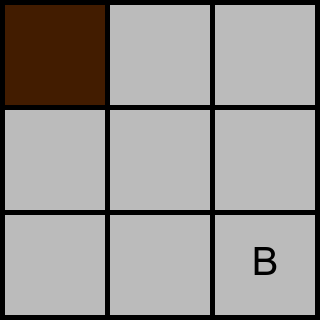
\includegraphics[width=\linewidth]{0.png}
\endminipage\hfill
\minipage{0.18\textwidth}
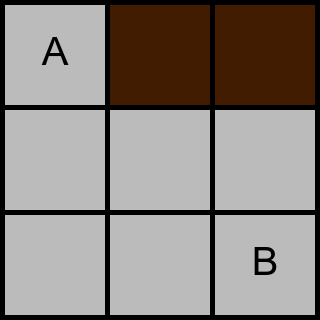
\includegraphics[width=\linewidth]{1.png}
\endminipage\hfill
\minipage{0.18\textwidth}
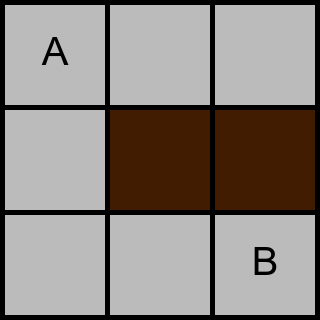
\includegraphics[width=\linewidth]{2.png}
\endminipage\hfill
\minipage{0.18\textwidth}
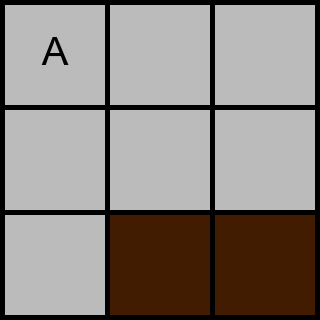
\includegraphics[width=\linewidth]{3.png}
\endminipage\hfill
\minipage{0.18\textwidth}
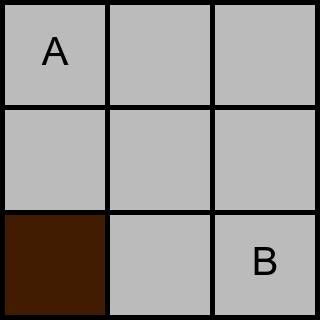
\includegraphics[width=\linewidth]{4.png}
\endminipage
\caption{Half of the solution to the first sample. The block is first moved one step to the right, then two steps down, and finally one step to the left.}
\end{figure}

\noindent On more advanced boards, so-called \emph{modulo cells} also appear. These are cells that can be in two different states, $0$ or $1$. In state $0$, a modulo cell behaves exactly like a free cell that the block can move on. In state $1$, however, modulo cells are raised and behave like blocked cells. There can also be toggle cells (marked with a $c$) placed on the board. When the block is placed on a toggle cell, the states of all modulo cells change ($0$ becomes $1$ and vice versa).

\begin{figure}[!htb]
\minipage{0.45\textwidth}
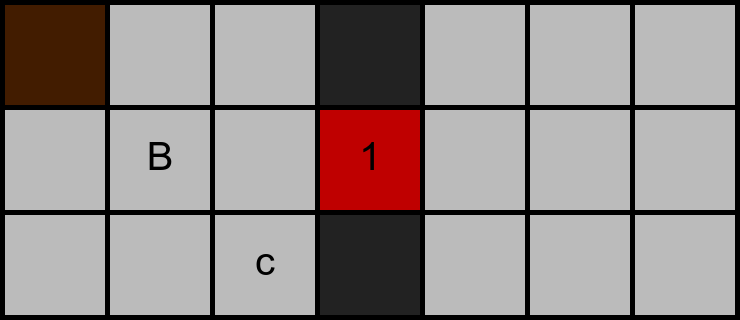
\includegraphics[width=\linewidth]{m0.png}
\endminipage\hfill
\minipage{0.45\textwidth}
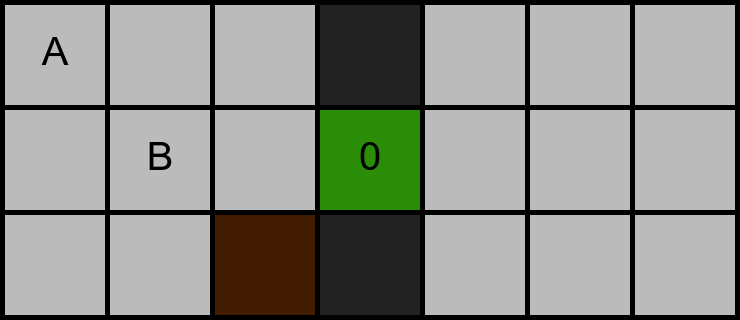
\includegraphics[width=\linewidth]{m1.png}
\endminipage
\caption{The third sample, before and after the toggle has been activated.}
\end{figure}

\noindent The boards are designed so that there is always a valid solution. Your task is to compute the minimum number of moves needed to solve a board.

\section*{Input}

You will first receive two integers $N$ and $M$. This means that the board has $N$ rows and $M$ columns.
The following $N$ lines have $M$ characters each and describe the board layout. The following characters may appear:

\begin{itemize}
\item $A$ or $B$: describes the board's start and end positions, respectively.
\item . (a period): describes a free cell.
\item \#: describes a blocked cell.
\item $0$ or $1$: describes a modulo cell with the given initial state.
\item c: describes a toggle cell.
\end{itemize}

It is guaranteed that each board contains exactly one $A$ and one $B$.

\section*{Output}

Output a single line with an integer, the minimum number of moves needed to move the block from cell $A$ to cell $B$.

\section*{Scoring}

For test cases worth 40 points, a board has at most $7$ rows and $7$ columns, but no modulo cells.

\noindent For the remaining 60 points, your solution also needs to handle modulo cells.
